\documentclass[12pt, dvipsnames]{report}

\usepackage{amsmath}
\usepackage{algorithm}
%\usepackage{algorithmic}
\usepackage[noend]{algpseudocode}

\usepackage{amsmath}
\usepackage{amssymb}
\usepackage{amsthm}
\usepackage{amsopn}

\usepackage{kpfonts}

\usepackage{graphicx}

% Probably don't need this on notes anymore
%\usepackage{kbordermatrix}

% Standard tool for drawing diagrams.
\usepackage{tikz}
\usepackage{tkz-berge}
\usepackage{tikz-cd}
\usepackage{tkz-graph}

\usepackage{comment}

%
\usepackage{multicol}

%
\usepackage{framed}

%
\usepackage{mathtools}

%
\usepackage{float}

%
\usepackage{subfig}

%
\usepackage{wrapfig}

%
\let\savewideparen\wideparen
\let\wideparen\relax
\usepackage{mathabx}
\let\wideparen\savewideparen

% Used for generating `enlightening quotes'
\usepackage{epigraph}

% Forget what this is used for :P
\usepackage[utf8]{inputenc}

% Used for generating quotes.
\usepackage{csquotes}

% Allows what to generate links inside
% generated pdf files
\usepackage{hyperref}

% Allows one to customize theorem
% environments in mathematical proofs.
\usepackage{thmtools}

% Gives access to a proof
\usepackage{lplfitch}

% I forget what this is for.
\usepackage{accents}

% A package for drawing simple trees,
% as a substitute for unnesacary TIKZ code
\usepackage{qtree}

% Enables sequent calculus proofs
\usepackage{ebproof}

% For braket notation
\usepackage{braket}

% To change line spacing when using mathematical notations which require some height!
\usepackage{setspace}

%\usepackage[dvipsnames]{xcolor}

\usepackage{float}

% For block commenting
\usepackage{comment}




\setlength\epigraphwidth{8cm}

\usetikzlibrary{arrows, petri, topaths, decorations.markings}

% So you can do calculations in coordinate specifications
\usetikzlibrary{calc}
\usetikzlibrary{angles}

\theoremstyle{plain}
\newtheorem{theorem}{Theorem}[chapter]
\newtheorem{axiom}{Axiom}
\newtheorem{lemma}[theorem]{Lemma}
\newtheorem{corollary}[theorem]{Corollary}
\newtheorem{prop}[theorem]{Proposition}
\newtheorem{exercise}{Exercise}[chapter]
\newtheorem{fact}{Fact}[chapter]

\newtheorem*{example}{Example}
\newtheorem*{proof*}{Proof}

\theoremstyle{remark}
\newtheorem*{exposition}{Exposition}
\newtheorem*{remark}{Remark}
\newtheorem*{remarks}{Remarks}

\theoremstyle{definition}
\newtheorem*{defi}{Definition}

\usepackage{hyperref}
\hypersetup{
    colorlinks = true,
    linkcolor = black,
}

\usepackage{textgreek}

\makeatletter
\renewcommand*\env@matrix[1][*\c@MaxMatrixCols c]{%
  \hskip -\arraycolsep
  \let\@ifnextchar\new@ifnextchar
  \array{#1}}
\makeatother

\renewcommand*\contentsname{\hfill Table Of Contents \hfill}

\newcommand{\optionalsection}[1]{\section[* #1]{(Important) #1}}
\newcommand{\deriv}[3]{\left. \frac{\partial #1}{\partial #2} \right|_{#3}} % partial derivative involving numerator and denominator.
\newcommand{\lcm}{\operatorname{lcm}}
\newcommand{\im}{\operatorname{im}}
\newcommand{\bint}{\mathbf{Z}}
\newcommand{\gen}[1]{\langle #1 \rangle}

\newcommand{\End}{\operatorname{End}}
\newcommand{\Mor}{\operatorname{Mor}}
\newcommand{\Id}{\operatorname{id}}
\newcommand{\visspace}{\text{\textvisiblespace}}
\newcommand{\Gal}{\text{Gal}}

\newcommand{\xor}{\oplus}
\newcommand{\ft}{\wedge}
\newcommand{\ift}{\vee}

\newcommand{\prob}{\mathbf{P}}
\newcommand{\expect}{\mathbf{E}}
\DeclareMathOperator{\Var}{\mathbf{V}}
\newcommand{\Ber}{\text{Ber}}
\newcommand{\Bin}{\text{Bin}}

%\newcommand{\widecheck}[1]{{#1}^{\ft}}

\DeclareMathOperator{\diam}{\text{diam}}

\DeclareMathOperator{\QQ}{\mathbf{Q}}
\DeclareMathOperator{\ZZ}{\mathbf{Z}}
\DeclareMathOperator{\RR}{\mathbf{R}}
\DeclareMathOperator{\HH}{\mathbf{H}}
\DeclareMathOperator{\CC}{\mathbf{C}}
\DeclareMathOperator{\AB}{\mathbf{A}}
\DeclareMathOperator{\PP}{\mathbf{P}}
\DeclareMathOperator{\MM}{\mathbf{M}}
\DeclareMathOperator{\VV}{\mathbf{V}}
\DeclareMathOperator{\TT}{\mathbf{T}}
\DeclareMathOperator{\LL}{\mathcal{L}}
\DeclareMathOperator{\EE}{\mathbf{E}}
\DeclareMathOperator{\NN}{\mathbf{N}}
\DeclareMathOperator{\DQ}{\mathcal{Q}}
\DeclareMathOperator{\IA}{\mathfrak{a}}
\DeclareMathOperator{\IB}{\mathfrak{b}}
\DeclareMathOperator{\IC}{\mathfrak{c}}
\DeclareMathOperator{\IP}{\mathfrak{p}}
\DeclareMathOperator{\IQ}{\mathfrak{q}}
\DeclareMathOperator{\IM}{\mathfrak{m}}
\DeclareMathOperator{\IN}{\mathfrak{n}}
\DeclareMathOperator{\IK}{\mathfrak{k}}
\DeclareMathOperator{\ord}{\text{ord}}
\DeclareMathOperator{\Ker}{\textsf{Ker}}
\DeclareMathOperator{\Coker}{\textsf{Coker}}
\DeclareMathOperator{\emphcoker}{\emph{coker}}
\DeclareMathOperator{\pp}{\partial}
\DeclareMathOperator{\tr}{\text{tr}}

\DeclareMathOperator{\supp}{\text{supp}}

\DeclareMathOperator{\codim}{\text{codim}}

\DeclareMathOperator{\minkdim}{\dim_{\mathbf{M}}}
\DeclareMathOperator{\hausdim}{\dim_{\mathbf{H}}}
\DeclareMathOperator{\lowminkdim}{\underline{\dim}_{\mathbf{M}}}
\DeclareMathOperator{\upminkdim}{\overline{\dim}_{\mathbf{M}}}
\DeclareMathOperator{\lhdim}{\underline{\dim}_{\mathbf{M}}}
\DeclareMathOperator{\lmbdim}{\underline{\dim}_{\mathbf{MB}}}
\DeclareMathOperator{\packdim}{\text{dim}_{\mathbf{P}}}
\DeclareMathOperator{\fordim}{\dim_{\mathbf{F}}}

\DeclareMathOperator*{\argmax}{arg\,max}
\DeclareMathOperator*{\argmin}{arg\,min}

\DeclareMathOperator{\ssm}{\smallsetminus}

\title{Complex Analysis}
\author{Jacob Denson}

\begin{document}

\pagenumbering{gobble}
\maketitle
\tableofcontents
\pagenumbering{arabic}

\chapter{Introduction}

The study of complex numbers is the analysis of a strange mathematical creation. Originally, these numbers were used as an `imaginary' mathematical creation used to find solutions to polynomial equations. However, in the early 19th century these numbers began being viewed as a geometric construction, another way to describe the two dimensional plane $\mathbf{R}^2$. The introduction of this number system on top of the plane has a much higher structure. And function differentiable with respect to this coordinate system has drastic differences to the study of complex numbers. It offers results many would described as miraculous and magical. What's more, the theory of complex analysis introduces many concepts which have formed the building blocks of many 20th century mathematical fields in topology, geometry, algebra, and analysis. In this first section, we introduce the complex numbers formally, as well as discussing the fundamental tools we will use in the study of complex analysis.

\section{The Complex Numbers}

As a numerical calculation system, the real numbers have many advantages: they are complete, enabling us to use Newton's calculus with precisious, as well as forming an ordered system of numbers, giving us a standard tool for comparing magnitudes which occur throughout the sciences. Nevertheless, the number system has one deficiency: there are some mathematical equations we are unable to solve. Since the square of every real number is positive, we cannot find a number $x$ which satisfies the equation $x^2 = -1$. The complex number system $\mathbf{C}$ is obtained by `imagining' a new number $i$, which does satisfy the equation $i^2 = -1$, and building a new number system containing $i$, and all real numbers, in such a way that most of the useful mathematical laws which hold for the real numbers continue to hold for all numbers in $\mathbf{C}$.

To be precise, we introduce the language of modern algebra. The algebraic rules in $\mathbf{R}$ we tend to use the most often are those which make $\mathbf{R}$ into a {\it field}. We define $\mathbf{C}$ to be the smallest set of numbers containing $\mathbf{R}$, as well as containing a new $i$ satisfying the equation $i^2 = -1$, while also forming a field. Since we must be able to add and multiply arbitrary numbers in $\mathbf{C}$, we must have numbers of the form $a + ib$, for each $a,b \in \mathbf{R}$, because we must be able to multiply each real number by $i$, and to add the result to a real number. Using the commutative and distributive law, we find that
%
\[ (a + ib) + (x + iy) = (a + x) + i(b + y) \]
\[ (a + ib)(x + iy) = (ax - by) + i(bx + ay) \]
%
so the operations of addition and multiplication are closed under these operations. What's more, every nonzero number of the form $z = x + iy$ also has an inverse of this form, because if we define the {\bf complex conjugate} $\overline{z} = x - iy$, we find that $z\overline{z} = x^2 + y^2$, which is a nonzero real number if either $x$ or $y$ is nonzero, and then
%
\[ z \frac{\overline{z}}{x^2 + y^2} = z \left[ \frac{x}{x^2 + y^2} + i \frac{-y}{x^2 + y^2} \right] = 1 \]
%
so the set of numbers expandable in the form $a + ib$ is exactly the {\it smallest} field containing $\mathbf{R}$ and $i$. Thus every complex number is formally expandable in this form. This expansion must be unique, because if $x + iy = a + ib$, then $(x - a) + i(y-b) = 0$, and if $y \neq b$, we conclude that $i = (a-x)/(y-b)$ is a real number, which is impossible, so we must have $y = b$, and then $x = a$ follows automatically. Thus a complex number $z = a + ib$ is uniquely defined by its real and complex parts $\Re(z) = a$ and $\Im(z) = b$. Summing up these results using the language of field theory, we say that $\mathbf{C}$ is the field extension of degree two obtained from $\mathbf{R}$ by solving the polynomial equation $x^2 = -1$. We also note that since the standard laws of arithmetic apply to the complex numbers, we find that the equations
%
\[ (a + ib) + (x + iy) = (a + x) + i(b + y) \]
\[ (a + ib)(x + iy) = ax + (ay + bx)i + (by)i^2 = (ax - by) + (ay + bx)i \]
%
can be used to formally define the complex numbers; We don't need to `assume' the existence of $\mathbf{C}$ as an axiom. We can instead construct it by placing certain arithmetical operations on $\mathbf{R}^2$, using the definitions above.

\section{Geometry of the Complex Plane}

Geometrically, the complex plane can be identified with $\mathbf{R}^2$. This leads to useful insight into the theorems of complex analysis. First off, it gives a topological structure to the class of complex numbers, which when viewed geometrically is called the complex {\it plane}. The $x$ and $y$ axis of the plane are called the {\bf real axis} and {\bf imaginary axis}. A novel result of the introductions of arithmetical operations to $\mathbf{R}^2$ is that the norm has a pleasant form. If we denote the norm of a complex number $z$ by $|z|$, then the value satisfies $|z|^2 = z\overline{z}$, and we call $|z| > 0$ the {\bf modulus} of the complex number $z$. Since
%
\[ |zw|^2 = zw \overline{zw} = z\overline{z} w \overline{w} = |z|^2|w|^2 \]
%
we find that $|zw| = |z||w|$ and $|\overline{z}| = |z|$. The modulus gives a complete metric space structure to the complex plane. We note the triangle inequality $|z + w| \leq |z| + |w|$, as well as the other useful inequalities
%
\[ |\Re(z)|, |\Im(z)| \leq |z|\ \ \ \ \ ||z| - |w|| \leq |z - w| \]
%
which are trivial to verify.

Geometrically, the arithmetical operations of the complex numbers become incredibly beautiful when we look at the numbers in their {\bf polar form}. Recall that any point on the plane $\mathbf{R}^2$ can be expressed in terms of an angle $\theta$ and a radius $r$. Looking ahead, we note that the complex exponential $e^{it}$ satisfies Euler's formula $e^{it} = \cos t + i \sin t$ (we will prove this rigorously later), so that is polar coordinates, the number with coordinates $r$ and $\theta$ is exactly $re^{i\theta}$. Because we have the addition formula $e^{i(x + y)} = e^{ix}e^{iy}$, we find that $re^{it}r'e^{it'} = (rr')e^{i(t + t')}$, so that multiplying too complex numbers dilates their radius multiplicatively, and rotates their angular coordinate additively. Multiplying a fixed complex number about the whole plane is geometrically just a rotation and a dilation in two dimensions. This shows that the arithmetic of complex numbers is not just an abstractly defined construction to satisfy a single algebraic equation; it has a purely geometric definition, which explains why complex analysis leads to such majestic geometrical results.

\section{Complex Functions and Holomorphicity}

The really interesting part of complex analysis begin when we start looking at complex-valued functions defined on subsets of the complex plane. Classically, we write such a function in the form $w = f(z)$, referring to the domain as the `$z$-plane', and the codomain as the `$w$-plane'. We will mostly be analyzing maps defined on {\bf domains} of the plane, that is, open, connected subsets of the plane.
%
%How do we visualize such a function? Is it fairly simple to visualize a real-valued function, defined on a subset of the real numbers, since the graph of such a function lies in two-dimensional space. For complex numbers, it is not so easy to see that the graph approach works, since the graph lies in four dimensional space. We can still analyze pieces of the functions which lie in the real axis. For instance, we can analyze the modulus, argument, real, and imaginary parts of a complex function separately.
%
%A more advanced and very modern way of analyzing a complex function is through {\bf domain colouring}. Via the colour wheel, we may identify every point on the complex plane by a certain colour and intensity. This is the trick which enables us to draw a four-dimensional complex function. At each point $z$, we draw the colour representing $f(z)$. You might not be able to draw this by hand, but if you are able to use a computer, it's a great visual tool.
%
%\begin{example}
%    Consider the function $w = z^2$. If we analyze the graph of the modulus $w = |z^2| = |z|^2$, we see that it is a paraboloid of revolution. The level curves are circles around the origin.
    %
%    \begin{center}
%    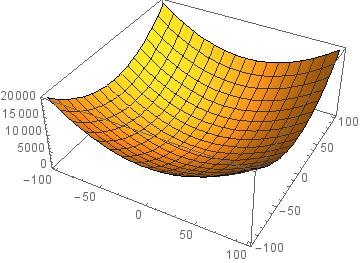
\includegraphics[scale = 0.3]{complexz2abssurface}
%    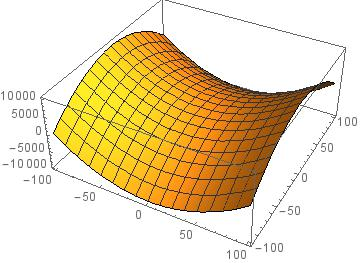
\includegraphics[scale = 0.3]{complexz2resurface}
%    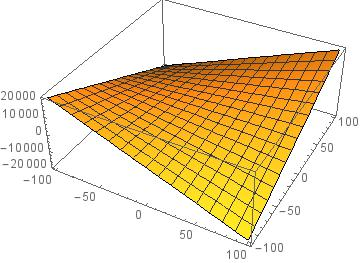
\includegraphics[scale = 0.3]{complexz2imsurface}

%    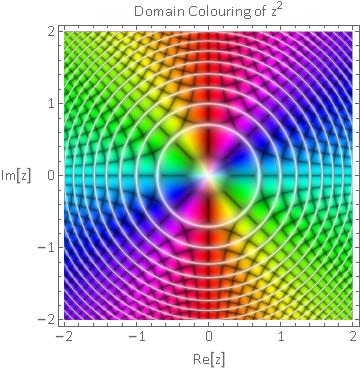
\includegraphics[scale = 0.5]{colorz2}
%    \end{center}
    %
%    The graph of the real part $w = \Re(z^2)$ can be written as $w = \Re(z)^2 - \Im(z)^2$. This is a hyperbololic paraboloid, as is the imaginary part can be written $w = 2\Re(z)\Im(z)$, with level curves
    %
%    \[ \Im(z) = \frac{w}{2 \Re(z)} \]
    %
%    Graphs of the three component functions are shown above.
%\end{example}
%
The standard definition of differentiability of real-valued functions generalizes easily to complex-valued functions, but the definition hides the fact that complex differentiability is a much stronger property than standard differentiability. A complex-valued function $f: \mathbf{C} \to \mathbf{C}$ is {\bf complex differentiable
}, {\bf holomorphic}, or {\bf regular} at $z$ if the limit
%
\[ \lim_{h \to 0} \frac{f(z + h) - f(z)}{h} \]
%
exists, which is now a value in the complex plane, denoted $f'(z)$. Unlike differentiability on the real plane, we note that complex differentiability is a much stronger condition on the local behaviour of $f$ around $z$. Whereas the real-valued limit can only by approached by two directions, complex differentiability is a limit approached from any approach trajectory. The set of all holomorphic functions defined on a domain $D$ is denoted $C^\omega(D)$. If $f$ is complex differentiable at $z$, then the limit implies exactly that we can write $f(z + w) = f(z) + w f'(z) + o(w)$. In terms of complex multiplication, that means that $f$ is locally just a translation, combined with a rotation and a dilation. The addition, multiplication, quotient, and chain rule continue to hold from normal calculus.

\begin{example}
    Every polynomial $f(z) = a_0 + a_1z + \dots + a_nz^n$ is differentiable at any point in the complex plane, with derivative $f'(z) = a_1 + 2a_2z + \dots + na_nz^{n-1}$. It is easy to see that the derivative of $w = z$ is $w' = 1$, and then the addition and product rule verifies the rule for all polynomials.
\end{example}

\begin{example}
    The function $w = 1/z$ is differentiable on $\mathbf{C} - \{ 0 \}$, because
    %
    \[ \lim_{h \to 0} \frac{(z + h)^{-1} - z^{-1}}{h} = \lim_{h \to 0} -\frac{1}{z(z+h)} = -\frac{1}{z^2} \]
\end{example}

\begin{example}
    The function $f(z) = \overline{z}$, though just a simple reflection in the complex plane, is not {\it complex} differentiable anywhere. This is because
    %
    \[ \lim_{h \to 0} \frac{\overline{z + h} - \overline{z}}{h} = \lim_{h \to 0} \frac{\overline{h}}{h} \]
    %
    And this limit does not exist, because if we approach the limit from the imaginary axis, with $h = ti$, then $\overline{h}/h = -1$, and if we approach the limit from the real axis, with $h = t$, then $\overline{h}/h = 1$. A reflection is not locally a rotation and a dilation.
\end{example}

We previously noted that complex multiplication corresponds to a rotation and a dilation. In particular, for each $w$, the map $T_w(z) = wz$ is a linear map from $\mathbf{C}$ to itself. Viewing $\mathbf{C}$ as $\mathbf{R}^2$, we see it has a matrix representation
%
\[ T_w = \begin{pmatrix} w_1 & w_2 \\ -w_2 & w_1 \end{pmatrix} \]
%
The function $f(z) = \overline{z}$, viewed as a function from $\mathbf{R}^2$ to $\mathbf{R}^2$, is certainly differentiable, and in fact, $C^\infty$. It is linear, with matrix representation
%
\[ \begin{pmatrix} +1 & 0 \\ 0 & -1 \end{pmatrix} \]
%
This cannot be put in the form $T_w$ for any $w$, which reflects the nonexistence of a complex derivative. Not all linear endomorphisms of the plane are homotheties. However, there are relations which guarantee a linear map to be a rotation and a dilation. In fact, the matrix representation above shows that a function $f = u + iv$ is complex differentiable at a point if and only if it is real differentiable, and
%
\[ \frac{\partial u}{\partial x} = \frac{\partial v}{\partial y}\ \ \ \ \ \frac{\partial u}{\partial y} = -\frac{\partial v}{\partial x} \]
%
These are known as the {\bf Cauchy-Riemann equations}. As an alternate viewpoint, we can also approach this purely from the complex perspective, something we will find often gives the most elegant arguments as we go deeper into complex analysis. If $f$ is complex differentiable at $z$, then
%
\[ f(z + w) = f(z) + f'(z)w + o(w) \]
%
so
%
\[ \frac{\partial f}{\partial x} = \lim_{t \to 0} \frac{f(z + t) - f(z)}{t} = \lim_{t \to 0} \frac{f'(z)t + o(t)}{t} = f'(z) \]
\[ \frac{\partial f}{\partial y} = \lim_{t \to 0} \frac{f(z + it) - f(z)}{t} = \lim_{t \to 0} \frac{itf'(z) + o(it)}{t} = if'(z) \]
%
If $f$ is complex differentiable, then we find
%
\[ \frac{\partial f}{\partial y} = i\frac{\partial f}{\partial x} \]
%
This is precisely the Cauchy Riemann equations in complex form.

\section{Integration Along Curves}

One distinguishing feature separating the study of complex analysis from Newton's one dimensional calculus is the reliance on line integration, which you may have encountered in multivariate calculus. Firstly, we will find ourselves not integrating over the whole complex plane, but instead integrating over curves lying in the complex plane. A {\bf smooth curve} is an immersion of a closed interval into $\mathbf{C}$ (viewing the interval as an oriented one dimensional manifold with boundary, and $\mathbf{C}$ as a two dimensional manifold). More simply, we define a {\bf smooth parameterization} $z: [a,b] \to \mathbf{C}$ to be a differentiable map whose derivative is continuous, and $z'(t) \neq 0$ for all $t \in [a,b]$, where we interpret $z'(a)$ and $z'(b)$ as the left and right hand limits
%
\[ \lim_{h \to 0^+} \frac{z(a + h) - z(a)}{h}\ \ \ \ \ \lim_{h \to 0^-} \frac{z(b + h) - z(b)}{h} \]
%
Two smooth curves $z_0: [a_0,b_0] \to \mathbf{C}$ and $z_1: [a_1,b_1] \to \mathbf{C}$ are {\bf equivalent} if there is a continuously differentiable function $s: [a_0,b_0] \to [a_1,b_1]$ with $s'(t) > 0$ for all $t$, such that $z_0(t) = z_1(s(t))$ for all $t \in [a_0,b_0]$. We then define a smooth curve to be an equivalence class of smooth parameterizations. More generally, a {\bf piecewise smooth curve} is an equivalence class of continuous parameterizations $z: [a,b] \to \mathbf{C}$, with values $a = a_0 < a_1 < \dots < a_n = b$ such that $z$ is a smooth curve on $[a_i,a_{i+1}]$, where $z_0: [a_0,b_0] \to \mathbf{C}$ and $z_1:[c_0,d_0] \to \mathbf{C}$ are equivalent if there are $a = a_0 < \dots < a_n = b$ and $c = c_0 < \dots < b_n = d$ such that $z_0$ and $z_1$ are equivalent on each of the intervals $[a_i,a_{i+1}]$ and $[c_i,c_{i+1}]$. This is a general enough class of curves for our purposes in complex analysis.

\begin{example}
    The standard example of a curve is the circle $C_r(z_0)$, of radius $r$ centered at $z_0$. The {\it positive orientation} of this curve is given by the parameterization
    %
    \[ z(t) = z_0 + re^{it} \]
    %
    On $[0,2\pi]$, and the {\it negative orientation}
    %
    \[ z(t) = z_0 + re^{-it} \]
    %
    also defined on $[0,2\pi]$. In general, we will interpret $C_r(z_0)$ as having the positive orientation. In particular, we denote $C_1(0)$ by $S^1$, the unit circle.
\end{example}

We will also need to introduce a couple more tools to manipulate curves. The {\bf inverse orientation} of a curve with parameterization $z: [a,b] \to \mathbf{C}$, which is the curve with parameterization $z^-: [a,b] \to \mathbf{C}$ with $z^-(t) = z(a+b-t)$. A curve $z: [a,b] \to \mathbf{C}$ is {\bf closed} if $z(a) = z(b)$, which means its image forms a `closed loop' in the plane. Now given a smooth curve $C$ with parameterization $z: [a,b] \to D$, where $D$ is some open subset of the complex plane, and a continuous function $f: D \to \mathbf{C}$, we define the {\bf line integral} of $f$ on $C$ as
%
\[ \int_C f(z) dz = \int_a^b f(z(t)) z'(t) dt \]
%
which we can remember by the mneumonic
%
\[ f(z) dz = f(z) \left( \frac{dz}{dt} \right) dt \]
%
so we can obtain the formula by `multiplying by a $dt/dt$ factor'. If $z'$ is only piecewise smooth, with partition $a_0 < \dots < a_n$, then we define
%
\[ \int_C f(z) dz = \sum \int_{a_i}^{a_{i+1}} f(z(t)) z'(t) dt \]
%
The change of variables formula for one dimensional integrals verifies that these definitions are independent of parameterization.

\begin{theorem}
    The line integral satisfies the following properties
    %
    \begin{itemize}
        \item For a given curve $C$ on some domain $D$, for any two $f,g \in C(D)$, $\alpha, \beta \in \mathbf{C}$,
        %
        \[ \int_C (\alpha f + \beta g)(z) dz = \alpha \int_C f(z) dz + \beta \int_C g(z) dz \]

        \item If $C^-$ is the reverse orientation of $C$, then
        %
        \[ \int_{C^-} f(z) dz = - \int_C f(z) dz \]

        \item One has
        %
        \[ \left| \int_C f(z) dz \right| \leq l(C) \| f \|_\infty \]
        %
        where $\| f \|_\infty$ is the supremum of $f$ over image of the curve $C$, and $l(C)$ is the {\bf length} of the curve $C$, defined to be the integral $\int_a^b |z'(t)| dt$.
    \end{itemize}
\end{theorem}
\begin{proof}
    The first theorem follows by the linearity of one dimensional integration by expanding out formulas, and the second theorem follows because $(z^-)'(t) = -z'(a+b-t)$. Finally, the third theorem follows because if $z: [a,b] \to \mathbf{C}$ is smooth, then
    %
    \[ \left| \int_C f(z)dz \right| = \left| \int_a^b f(z(t)) z'(t) dt \right| \leq \int_a^b |f(z(t))||z'(t)| dt \leq \| f \|_\infty \int_a^b |z'(t)| dt \]
    %
    and the result for piecewise smooth curves follows by linearity.
\end{proof}

Finally in our review of line integration, we recall a very useful result. We say a function $f: D \to \mathbf{C}$ on some domain $D$ has a {\bf primitive} if there is a function $F: D \to \mathbf{C}$ holomorphic on $D$ such that $F'(z) = f(z)$.

\begin{theorem}
    If $f$ is continuous, and has a primitive $F$ on $D$, then a curve $C$ begining at $z$ and ending at $w$ has
    %
    \[ \int_C f(z)dz = F(w) - F(z) \]
    %
    In particular, if $C$ is a closed curve in $D$, then $\int_C f(z)dz = 0$.
\end{theorem}
\begin{proof}
    If $C$ is smooth, then
    %
    \[ \int_C f(z)dz = \int_a^b f(z(t)) z'(t) dt \]
    %
    Now if $F'(z) = f(z)$ for each $z \in D$, then the chain rule (which is easily proved for compositions of functions from intervals to $\mathbf{C}$ and from holomorphic functions on $\mathbf{C}$) implies that $(F \circ z)'(t) = F'(z(t)) z'(t)$, and therefore the fundamental theorem of calculus (applied componentwise on the integral of the complex valued function $f(z(t)) z'(t)$), we conclude that
    %
    \[ \int_a^b f(z(t)) z'(t) dt = F(z(b)) - F(z(a)) = F(w) - F(z) \]
    %
    The theorem is then proved for piecewise smooth curves by a telescoping summation.
\end{proof}

\begin{corollary}
    If $f$ is a holomorphic function on a domain $D$ with $f' = 0$, then $f$ is constant on $D$.
\end{corollary}
\begin{proof}
    If $z$ and $w$ are two points on $D$, let $C$ be a smooth curve beginning at $z$ and ending at $w$. Then since $f' = 0$,
    %
    \[ \int_C f'(z) dz = 0  \]
    %
    But also since $f'$ has a primitive $f$, we find that
    %
    \[ \int_C f'(z) dz = f(w) - f(z) \]
    %
    and hence $f(w) = f(z)$.
\end{proof}

\begin{example}
    The function $f(z) = 1/z$ does not have a primitive in $\mathbf{C} - \{ 0 \}$, where it is defined, because
    %
    \[ \int_{S^1} \frac{dz}{z} = \int_0^{2\pi} \frac{ie^{it}}{e^{it}} = \int_0^{2\pi} i = 2 \pi i \]
    %
    Whereas if $1/z$ did have a primitive, we would conclude this integral is zero. We shall find that this is the essential holomorphic function without a primitive.
\end{example}














\section{Riemann Surfaces}

The study of differentiable manifolds generalizes the calculus of real variables in Euclidean space to spaces which locally behave like Euclidean space. In this section we discuss the theory which generalizes the theory of holomorphic functions on domains in the complex plane to spaces which locally behave like the complex plane. These `one-dimensional complex manifolds' are known as {\bf Riemann surfaces}. Topological intuition suggests that complex manifolds should be 2-dimensional real manifolds, with additional structure which enables us to identify a class of holomorphic functions. The standard way to identify differentiable functions on a real manifold is to introduce a $C^\infty$ structure, considering an atlas of local embeddings $x: U \to \mathbf{R}$, such that if $y: V \to \mathbf{R}$ is any other embedding, the transition map $x \circ y^{-1}$ is $C^\infty$ where defined. Similarily, we introduce a {\bf $C^\omega$ atlas} to be a cover of a two dimensional manifold by charts such that any two chars $(x,U)$ and $(y,V)$ have a holomorphic transition map $x \circ y^{-1}$ where defined. A two dimensional manifold $M$ with a fixed $C^\omega$ atlas is known as a Riemann surface.

Every Rieman surface $M$ is certainly a two dimensional manifold, so we can consider the tangent space $T_p M$. What's more, we can give these two dimensional tangent spaces a one dimensional complex structure. Recall that if $V$ is an $\mathbf{R}$ vector space, and $J: V \to V$ is a linear map such that $J^2 = -1$, then we may make $V$ into a complex vector space by defining $(a + bi)v = a + bJv$, so that a complex vector space is just a real vector space with a fixed `90 degree rotation'. We define a family of linear maps $J_p: T_p M \to T_p M$ at each point by use of the holomorphic coordinates. If $(x,U)$ is a chart at $p$, then we may write each tangent vector $v$ at $p$ in the coordinates of $x$ with a unique $z \in \mathbf{C}$, by the correspondence $x_*$. We define $Jv$ in the coordinates of $x$ to be $iz$. If $y$ is another chart at $p$, then $v$ has coordinates $(y \circ x^{-1})'(x(p)) \cdot z$, and $Jv$ has coordinates $(y \circ x^{-1})'(x(p))(iz) = i(y \circ x^{-1})'(x(p)) z$. Precisely because the transition map is holomorphic, the multiplication by $i$ is invariant of being taken inside brackets or outside brackets. This means $J$ is independant of the coordinate system, and so the tangent spaces are one-dimensional complex vector spaces.

A map $f: M \to N$ between Riemann surfaces is holomorphic if the map is holomorphic in every coordinate system. Since we have the tangent bundle, there is a more natural coordinate-invariant definition. Provided $f$ is differentiable (which it must be if it is holomorphic), $f$ induces a map $f_*: TM \to TN$. $f$ is holomorphic at a point if and only if $f_*$ is complex-linear at the point. This makes sense, because Riemann surfaces should model the local properties of the complex plane, and holomorphic functions on the complex plane are exactly those functions which are locally complex linear maps.

\begin{example}
    The fundamental example of a Riemann surface is the Riemann sphere $\mathbf{C}^\infty = \mathbf{C} \cup \{ \infty \}$, whose topology is defined to be the compactification of $\mathbf{C}$. The subsets $\mathbf{C}$ and $\mathbf{C}^\infty - \{ 0 \}$ both have homeomorphisms onto $\mathbf{C}$, the first by the identity map, and the second by the map $z \mapsto 1/z$. The maps are compatible since $1/z$ is holomorphic for $z \neq 0$ on $\mathbf{C}$. A function $f: \mathbf{C}^\infty \to \mathbf{C}$ is holomorphic if and only if $f(z)$, and $f(1/z)$ are holomorphic. Life is more fun when we can consider holomorphic functions from $\mathbf{C}$ to $\mathbf{C}^\infty$, which are meromorphic functions, and holomorphic functions from $\mathbf{C}^\infty$ to $\mathbf{C}^\infty$, which are meromorphic functions meromorphic at $\infty$.
\end{example}

Fundamentally, the `$J$' map is what defines the holomorphic properties of a $2$-manifold. If a given bundle map $J:TM \to TM$ is given such that $J^2 = -1$, then this map defines a complex linear structure on the tangent spaces, and we define $f: M \to N$ to be holomorphic if the corresponding map $f_*$ is complex linear at each point. A holomorphic atlas on $M$ may then be define to be the set of all `holomorphic charts', for if $(x,U)$ and $(y,V)$ are holomorphic charts, then $x \circ y^{-1}$ is holomorphic, for it is certainly differentiable, and the derivative is complex linear. Thus as long as $J$ is `consistant', in the sense that there exist enough holomorphic charts to cover the manifold, then $J$ is a perfectly reasonable way to define a complex structure on a $2$-manifold. In fact, $J$ is what we call a {\bf almost complex structure} on the manifold, for it is almost all we need to define holomorphic functions.

Even if we forget the tangent space $T_p M$, we may still reconstruct it from a holomorphic atlas by considering derivations. Recall that a $p$-derivation is a complex-valued function $\Lambda$ such that for any two functions $f,g \in C^\infty(M,\mathbf{C})$, $\Lambda (fg) = f(p) \Lambda g + g(p) \Lambda f$. The differential operators $\partial_x$ and $\partial_y$ are contained in $T_p \mathbf{C}$, and the same argument as in the real case shows these operators span the complex vector space of all derivations. As with a tangent space, we can consider the cotangent space $T_p^* \mathbf{C}$, the dual space of $T_p \mathbf{C}$. A smooth $f: \mathbf{C} \to \mathbf{C}$ gives rise to a section $df$ of the cotangent space, and $dx(p)$ and $dy(p)$ span the cotangent space at each point.

The most intriguing part of this construction occurs when we examine holomorphic functions. In classic notation, define $z$ to be the identity map on $\mathbf{C}$. Then $z$ is trivially smooth, and so we may consider $dz = dx + i dy$. Define $\overline{z} : w \to \overline{w}$. Then $d\overline{z} = dx - i dy$. These equations are linearly independant, and thus span the cotangent space at each point. Thus any $w \in T_p^* \mathbf{C}$ may be written $\alpha dz + \beta d\overline{z}$ for two values $\alpha$ and $\beta$. In particular, this holds for $df$. We define the coefficients $\partial_z f$ and $\partial_{\overline{z}} f$ by the equation $df = \partial_z f dz + \partial_{\overline{z}} f d\overline{z}$. Since $\alpha dz + \beta d\overline{z} = (\alpha + \beta) dx + i(\alpha - \beta) dy$. We obtain the equalities
%
\[ \frac{\partial f}{\partial z} + \frac{\partial f}{\partial \overline{z}} = \frac{\partial f}{\partial x}\ \ \ \ \ \frac{\partial f}{\partial z} - \frac{\partial f}{\partial \overline{z}} = -i \frac{\partial f}{\partial y} \]
%
Reordering these equations, we determine that
%
\[ \frac{\partial f}{\partial z} = \frac{1}{2} \left( \frac{\partial f}{\partial x} - i \frac{\partial f}{\partial y} \right)\ \ \ \ \ \frac{\partial f}{\partial \overline{z}} = \frac{1}{2} \left( \frac{\partial f}{\partial x} + i \frac{\partial f}{\partial y} \right) \]
%
If $f$ is real-differentiable at a point $z$, then
%
\[ f(z + w) = f(z) + w \left. \frac{\partial f}{\partial z} \right|_z + \overline{w} \left. \frac{\partial f}{\partial \overline{z}} \right|_z + o(w) \]
%
so these partial derivatives separate the parts of the derivative as the part corresponding to the identity and the parts corresponding to the conjugate. This is possible because the space of real-linear endomorphisms on $\mathbf{C}$ is four dimensional, and each of the partial derivatives in the equation above has two degrees of freedom.

Note that the Cauchy Riemann equations state exactly that $\partial_{\overline{z}} f = 0$, and $f' = \partial_z f$. This explains why the operators $\partial_{\overline{z}}$ rarely come up once we discuss holomorphic functions. And indeed, we find that the `tangent space' corresponding to the space of holomorphic functions is one dimensional, spanned by $\partial_z$. Since the space of holomorphic functions does not contain bump functions, simply taking derivations on $C^\omega(\mathbf{C})$ would not be local enough to correspond to a tangent space. Thus we define the tangent space to be the space of derivations on the algebra $A$ of germs of holomorphic functions defined in a neighbourhood of a point.

\begin{theorem}
    The derivations on $A$ are multiples of $\partial_z$.
\end{theorem}
\begin{proof}
    Without loss of generality, assume the point is the origin. Let $l$ be a derivation. If $f$ is holomorphic, then $g(z) = (f(z) - f(0))/z$ is holomorphic with $g(0) = f'(0)$, and we calculate $l(f) = l(gz) + f(0)l(1) = f'(0)l(z)$. This means that $l = l(z) \partial_z$.
\end{proof}

This also means that the cotangent space is spanned by $dz$. Since $dz(\dot{\gamma}(t)) = \gamma'(t)$, the differential forms definition of integration gives
%
\[ \int_\gamma f(z)\; dz = \int_a^b f(\gamma(t)) dz \left(\dot{\gamma}(t) \right)\; dt = \int_a^b f(\gamma(t)) \gamma'(t)\; dt \]
%
which is precisely the definition of contour integration we gave before. By linearity, all the real theorems on integration extend by linearity to this complex situation. In particular, Poincare's theorem implies that if $D$ is a simply connected domain, and $f$ is a smooth holomorphic function, then $dg = f dz$ for some function $g$, and so for any curve $\gamma$,
%
\[ \int_\gamma f\; dz = g(\gamma(b)) - g(\gamma(a)) \]
%
so if $\gamma$ is a closed curve, $\int_\gamma f\; dz = 0$. We will soon prove all holomorphic functions are smooth, so this very easily justifies generalizations of Cauchy's theorem to curves in simply connected regions.



\section{Power Series}

Polynomials are the simplest examples of holomorphic functions. Our next family of holomorphic functions will be obtained by taking limits of polynomials. In fact, we will soon show that this family essentially contains all holomorphic functions. We define a (formal) {\it power series} about a point $z_0$ is an `infinite dimensional polynomial'
%
\[ \sum_{n = 0}^\infty c_n (z - z_0)^n \]
%
We may evaluate a power series to obtain a function $f$, defined as
%
\[ f(z) = \sum_{k = 0}^\infty a_k (z - z_0)^k \]
%
whose domain is the set where the series converges. A function $f$ can be {\bf expanded in a power series} at a point $z_0$ if we may write $f$ as a power series locally around $z_0$. An {\bf analytic} function is a function which can be locally expanded as a power series at every point in its domain.

Standard tricks from real power series come into play here, and the proofs go unedited. The most useful is the root test, or Cauchy-Hadamard theorem, which states that, if we define
%
\[ 1/R = \limsup_{n \to \infty} |c_n|^{1/n} \]
%
Then the power series $f$ converges locally uniformly for $|z - z_0| < R$, and diverges for $|z - z_0| > R$. It may sometimes be easier to apply the ratio test. If the limit
%
\[ 1/L = \lim_{n \to \infty} \left| \frac{c_{n+1}}{c_n} \right| \]
%
exists, then $f$ converges for $|z - z_0| < L$, and diverges for $|z - z_0| > L$. These statements do not say anything about what happens on the boundary, when $|z - z_0|$ is equal to $R$ or $L$.

\begin{example}
    The most important power series, and perhaps the most important function in mathematics, is the exponential function, defined at all points in the complex plane by the fomrula
    %
    \[ e^z = \exp(z) = \sum_{n = 0}^\infty \frac{z^n}{n!} \]
    %
    Which converges by the ratio test, since $(n+1)!/n! = n \to \infty$. The product formula shows
    %
    \begin{align*}
    \exp(z + w) &= \sum_{k = 0}^\infty \frac{(z + w)^k}{k!} = \sum_{k = 0}^\infty \sum_{j = 0}^k \binom{k}{j} \frac{z^j w^{k-j}}{k!}\\
    &= \sum_{k = 0}^\infty \sum_{j = 0}^k \frac{z^j}{j!} \frac{w^{k-j}}{(k - j)!} = \exp(z) \exp(w)
    \end{align*}
    %
    which gives us the multiplicative property of the function.
\end{example}

\begin{example}
    The hypergeometric series is defined for $\alpha, \beta \in \mathbf{C}$, and $\gamma$ not a negative integer by
    %
    \[ F(\alpha,\beta,\gamma;z) = \sum_{n = 1}^\infty \frac{\alpha(\alpha+1)\dots(\alpha + n - 1) \beta(\beta + 1) \dots (\beta + n - 1)}{\gamma (\gamma + 1) \dots (\gamma + n - 1)} \frac{z^n}{n!} = \sum_{n = 1}^\infty \frac{(\alpha)_n (\beta)_n}{(\gamma)_n} \frac{z^n}{n!} \]
    %
    The notation $(\cdot)_n$ is known as a Pockhammer symbol. We calculate
    %
    \begin{align*}
        \log \left( \prod_{m = 0}^{N-1} (\lambda + m) \right) &= \sum_{m = 0}^{N-1} \log(\lambda + m) = \int_\lambda^{\lambda + N} \log x\; dx + O(\log(\lambda + N))\\
        &= N \log(\lambda + N) + O(\log(\lambda + N)) = N \log(N) + O(\log(\lambda + N))
    \end{align*}
    %
    In particular, $\log(N!) = N \log N + O(\log N)$. This means
    %
    \[ \log \left( \left( \frac{(\alpha)_n (\beta)_n}{(\lambda)_n} \frac{1}{n!} \right)^{1/n} \right) = \frac{O(\log(\alpha + \beta + \lambda + n))}{n} = o(1) \]
    %
    so
    %
    \[ \left( \frac{(\alpha)_n (\beta)_n}{(\lambda)_n} \frac{1}{n!} \right)^{1/n} \to 1 \]
    %
    so the series has a radius of convergence of one.
\end{example}

\begin{example}
    If we define the Bessel function
    %
    \[ J_m(z) = (z/2)^m \sum_{n = 0}^\infty \frac{(-1)^n}{n! (n+m)!} \]
    %
    Then we calculate
    %
    \begin{align*}
        \log \left( \left( \frac{1}{2^{2n} n! (n+m)!} \right)^{1/2n} \right) &= \frac{-2n \log 2 - 2n \log n + O(\log(n+m))}{2n}\\
        &= - \log 2 - \log n + o(1) \to -\infty
    \end{align*}
    %
    so $J_m$ is defined by a power series everywhere.
\end{example}

Calculus tells us that the derivative of the exponential function is the exponential function itself. If there is any justice in the world, this idea should extend to the complex case. We can formally calculate
%
\[ \exp'(z) = \sum_{k = 0}^\infty \left( \frac{z^k}{k!} \right)' = \sum_{k = 1}^\infty \frac{z^{k-1}}{(k-1)!} = \sum_{k = 0}^\infty \frac{z^k}{k!} = \exp(z) \]
%
But how do we know that the derivative of the power series can be obtained by differentiating each term in the series?

\begin{theorem}
    Let $f(z) = \sum_{k = 0}^\infty c_k z^k$ be a power series, convergent inside a disk $D$. Then $f$ is holomorphic in $D$, and $f'(z) = \sum_{k = 1}^\infty k c_k z^{k-1}$.
\end{theorem}
\begin{proof}
    The fact that the power series defining $f'$ converges in $D$ follows from the Hadamard formula. Now let us verify that this series, which defines a function $g$, approaches the derivative of $f$. Define $S_n$ to be the finite polynomial of degree $n$ defined by $f$, $S_n(z) = \sum_{k = 0}^n c_k z^k$. Let $E_n$ denote the error term, $E_n(z) = \sum_{k = n+1}^\infty c_k z^k$. Then $S_n'(z) = \sum_{k = 1}^n k c_k z^{k-1}$, and
    %
    \[ \frac{f(z + w) - f(z)}{w} = \left[ \frac{S_n(z + w) - S_n(z)}{w} - S_n'(z) \right] + \left[ \frac{E_n(z + w) - E_n(z)}{w} \right] + S_n'(z) \]
    %
    The first term converges to zero for small enough $w$. The third term converges to $g(z)$ as $n \to \infty$. The only tricky component is the second term. Since $a^n - b^n = (a - b)(a^{n-1} + a^{n-2}b + \dots + ab^{n-2} + b^{n-1})$. If we choose $|z|, |z + w| < r - \varepsilon$, then
    %
    \begin{align*}
        \left| \frac{E_n(z + w) - E_n(z)}{w} \right| &= \left| \sum_{k = n + 1}^\infty c_k \frac{(z + w)^k - z^k}{w} \right| \leq \sum_{k = n + 1}^\infty k |c_k| (r - \varepsilon)^{n-1}
    \end{align*}
    %
    The right side is a convergent power series, and hence as $n \to \infty$, the term converges to zero. By picking $n$ large enough, and $|z - w|$ small enough, the value can be made as close to $g$ as possible.
\end{proof}

\begin{corollary}
    A function $f(z) = \sum_{i = 0}^\infty c_i z^i$ expandable in a power series about a point has holomorphic derivatives $f', f'', f^{(3)}, \dots$ around the point, which are also expandable in a power series, with
    %
    \[ f^{(n)}(z) = \sum_{k = n}^\infty \frac{k!}{(k - n)!} c_k z^{k-n} \]
\end{corollary}

\begin{corollary}
    Every analytic function is holomorphic.
\end{corollary}

\section{Harmonic Functions}

A function $f: \mathbf{R}^2 \to \mathbf{C}$ is known as harmonic if
%
\[ \Delta f = \frac{\partial^2 f}{\partial x^2} + \frac{\partial^2 f}{\partial y^2} = 0 \]
%
We now discuss a connection which allows us to reduce their study to the study of holomorphic functions. We calculate
%
\[ \partial_z \partial_{\overline{z}} = \frac{(\partial_x - i \partial_y)(\partial_x + i \partial_y)}{4} = \frac{\partial^2_x + i \partial_x \partial_y - i \partial_y \partial_x + \partial_y^2}{4} = \frac{\Delta}{4} \]
%
So any holomorphic or antiholomorphic function is harmonic, as is it's real and imaginary part. Conversely, suppose that $g$ is a real-valued harmonic function. Then $\partial_{\overline{z}} \partial_z g = 0$, so $\partial_z g$ is holomorphic. We will later find that any holomorphic locally has an antiderivative, so in particular, we can find a holomorphic function $f$ with $f' = 2 \partial_z g$. But this means that
%
\[ \partial_x f_0 - i \partial_y f_0 = f' = 2 \partial_z g = \partial_x g - i \partial_y g \]
%
so $\nabla f_0 = \nabla g$, implying $f_0$ and $g$ differ by a constant. Patching the $f_0$ together shows that $g$ is the real part of a holomorphic function.

In particular, this implies that for any circle $C_r(z_0)$,
%
\[ 2 \pi i f(z_0) = \int_{C_r(z_0)} \frac{f(z)}{z - z_0}\; dz = i \int_0^{2\pi} f(z_0 + r e^{it})\; dt  \]
%
Taking the imaginary parts on both sides gives
%
\[ 2 \pi g(z_0) = \int_0^{2\pi} f(z_0 + e^{it})\; dt \]
%
So any harmonic function satisfies the mean value formula; the average value of the function around a circle is the same as the value of that function at the centre of the circle. Note that this is not necessarily true for the average of the function over every curve, since in the calculations above the imaginary parts of $f$ might contribute to the imaginary part of the integral.







\chapter{Cauchy's Theorem}

Cauchy's theorem says that the integral of a holomorphic function about a closed curve is always zero. This is simple, but forms the backbone for the theory of holomorphic functions. Originally, certain regularity were assumed on holomorphic functions to obtain Cauchy's theorem. But it was later discovered that one can obtain Cauchy's theorem assuming only that the function is holomorphic at each point in the region, and it is this procedure we will use to show the regularity of holomorphic functions completely.

\begin{theorem}[Goursat's lemma]
    If $T$ is a triangle, and $f$ is holomorphic in an open set containing the triangle and it's interior, then
    %
    \[ \int_T f(z)\; dz = 0 \]
\end{theorem}
\begin{proof}
    We can split the triangle $T$ into four smaller triangles $A$, $B$, $C$, and $D$, each with a quarter of the diameter and length. Since
    %
    \[ \int_T f(z)\; dz = \left( \int_{A} f(z)\; dz + \int_B f(z)\; dz + \int_C f(z)\; dz + \int_D f(z)\; dz \right) \]
    %
    We may choose one such triangle $T_1$ with
    %
    \[ \left| \int_{T_1} f(z)\; dz \right| \geq \left| \int_T f(z)\; dz \right| \]
    %
    Continuing inductively, we can find a nested family of rectangles $T_1 \supset T_2 \supset \dots T_n$ with $\text{diam}(T_n) = \text{diam}(T)/4^n$, $l(T_n) = l(T)/4^n$, and
    %
    \[ \left| \int_{T_n} f(z)\; dz \right| \geq 4^{-n} \left| \int_T f(z)\; dz \right| \]
    %
    As $n \to \infty$, $\text{diam}(T_n) \to 0$, so $\bigcap T_n$ contains a unique point $z_0$. We can write $f(z) = f(z_0) + f'(z_0) (z - z_0) + \psi(z - z_0)(z - z_0)$, with $\psi(w) \to 0$ as $w \to 0$. Now it is easy to calculate that
    %
    \[ \int_{T_n} f(z_0)\; dz = f'(z_0) \int_{T_n} (z - z_0)\; dz = 0 \]
    %
    so
    %
    \begin{align*}
        \left| \int_T f(z)\; dz \right| \leq 4^n \left| \int_{T_n} f(z)\; dz \right| &= 4^n \left| \int_{T_n} \psi(z-z_0)(z - z_0)\; dz \right|\\
        &\leq 4^n o(1) l(T_n) \text{diam}(T_n) = o(1/4^n)
    \end{align*}
    %
    and thus as $n \to \infty$, we conclude the integral over the triangle is zero.
\end{proof}

%TODO: INSERT DIAGRAMS HERE

Attaching two triangles together, we can obtain Cauchy's theorem for a rectangle. Given a holomorphic function $f$ on a circle, by defining $F(w)$ to be the line integral from the centre of the circle to $w$ on either half of the rectangle parallel to the axis, we find a function $F$ with $F' = f$, so $f$ has an integral, and Cauchy's theorem holds in a circle. More generally, this holds for any region where we can unambiguously construct rectangular arcs from one point to another. In particular, Cauchy's theorem holds for the `keyhole' curve (one can see that two rectangular arcs between points are equal by breaking them into rectangles if the arcs don't cross or self intersect, and by induction, assume the curves dont intersect by breaking them into smaller curves). Taking the keyhole smaller and smaller, we determine that if $f$ is holomorphic on the region between two circles, one containing the other, then the line integral over these two circles is equal to one another. This is very useful in proving the following integral formula for holomorphic functions.

\begin{theorem}
    If $f$ is holomorphic in a disc $D$ containing a point $w$, then
    %
    \[ f(w) = \frac{1}{2 \pi i} \int_{\partial D} \frac{f(z)}{z - w}\; dz \]
\end{theorem}
\begin{proof}
    Since $g(z) = f(z)/(z-w)$ is holomorphic everywhere in $D$ except at $w$, the integral over the entire circle is equal to the integral of an arbitrary small circle $C_\varepsilon(w)$ of radius $\varepsilon$ centered at $w$. We have
    %
    \[ \frac{f(z)}{z - w} = \frac{f(w)}{z - w} + O(1) \]
    %
    so
    %
    \[ \int_{C_\varepsilon(w)} \frac{f(z)}{z - w} = \int_{C_\varepsilon(w)} \frac{f(z)}{z-w} + O(\varepsilon) = i \int_0^{2\pi} f(z) e^{-it} e^{it} + O(\varepsilon) = 2 \pi i f(z) + O(\varepsilon) \]
    %
    We then take $\varepsilon \to 0$ to prove our theorem.
\end{proof}

\begin{remark}
Integral representation formulas are very important in analysis, because they enable us to control a function from its behaviour on a very small set, and also use it to show the function is suitably regular.
\end{remark}

\section{Consequences of Cauchy's Formula}

A simple corollary of Cauchy's integral formula, proved by induction, shows any holomorphic function is completely smooth.

\begin{theorem}
    If $f$ is holomorphic in a disk $D$, then $f$ has derivatives of all orders in $D$, with
    %
    \[ f^{(n)}(z) = \frac{n!}{2 \pi i} \int_{\partial D} \frac{f(z)}{(z - w)^{n+1}}\; dz \]
\end{theorem}
\begin{proof}
    We know this is true for $n = 0$. And now by induction, if it is true for $n$, then
    %
    \begin{align*}
        \frac{n!}{2 \pi i} \int_{\partial D} & \left( \frac{f(z)}{(z - w)^{n+1}} - \frac{f(z)}{(z - w_0)^{n+1}} \right)\; dz\\
        &= \frac{n!}{2 \pi i} \int_{\partial D} \frac{f(z)}{w_0 - w} \left( \frac{1}{z - w} - \frac{1}{z - w_0} \right) \left( \sum_{k = 0}^n \frac{1}{(z - w)^{n-k}(z - w_0)^k} \right)\\
        &= \frac{n!}{2 \pi i} \int_{\partial D} \frac{f(z)}{(z - w)(z - w_0)} \left( \sum_{k = 0}^n \frac{1}{(z - w)^{n-k}}(z - w_0)^k \right)
    \end{align*}
    %
    and as $w \to w_0$, we conclude that
    %
    \[ f^{(n+1)}(w_0) = \frac{(n+1)!}{2 \pi i} \int_{\partial D} \frac{f(z)}{w_0} \frac{1}{(z - w_0)^{n+2}} \]
\end{proof}

\begin{remark}
    Because of this, we obtain that for each $z$ in some disc $D$ upon which $f$ is holomorphic,
    %
    \[ \| f^{(n)}(z) \| \leq \frac{n! \| f \|_{L^\infty(\partial D)}}{d(z,\partial D)^n} \]
    %
    a result known as Cauchy's inequality. 
\end{remark}

Another regularity property enables us to show every holomorphic function is analytic, because
%
\[ \frac{1}{z - w} = \frac{1}{(z - z_0 - (w - z_0))} = \sum_{n = 0}^\infty \frac{(w - z_0)^n}{(z - z_0)^{n+1}} \]
%
which converges uniformly on $\partial D$, hence we can interchange integration and summation to obtain a power series representation of $f$ from Cauchy's integral formula. For the next theorem, one needs to know that an {\bf entire} function is one which is holomorphic on the entire complex plane.

\begin{theorem}[Louville]
    Every bounded and entire function is constant.
\end{theorem}
\begin{proof}
    Consider Cauchy's inequality for $n = 1$, which we just proved. As we take the radius of the disc $D$ to $\infty$, the term $\| f \|_{L^\infty(\partial D)}$ remains bounded, so the numerator is bounded, whereas the denominator tends to $\infty$ for every $z$. Thus we conclude $f' = 0$, so $f$ is constant.
\end{proof}

\begin{theorem}[The Fundamental Theorem of Algebra]
    Every nonconstant polynomial over the complex numbers has a root.
\end{theorem}
\begin{proof}
    Let $f$ be a polynomial with no root over the complex numbers. If $f$ has degree $n$, then for large $z$, $f(z) = (1 + o(1))z^n$. Thus $1/f(z)$ is an entire function, and it is also bounded, since $|z|^n \lesssim |f(z)|$ for large $n$. Thus $1/f(z)$ is constant, so $f$ is constant.
\end{proof}

\begin{theorem}[Morera]
    If $f$ is a function with $\int_T f(z)\; dz = 0$ for all triangles $T$ in a region, then $f$ is holomorphic.
\end{theorem}
\begin{proof}
    Then we know there is a primitive function $F$ with $F' = f$. But $F$ is holomorphic, hence infinitely differentiable, and so $f$ must also be infinitely differentiable.
\end{proof}

\section{Uniqueness of Holomorphic Functions}

\begin{theorem}
    Let $f$ be a holomorphic function, with $z_n \to w$ with $f(z_n) = 0$. Then $f = 0$ everywhere.
\end{theorem}
\begin{proof}
    Without loss of generality, assume $w = 0$. Write $f(z) = \sum_{n = 0}^\infty a_n z^n$ for $z$ close enough to zero. By continuity, $f(0) = a_0 = 0$. If $N > 0$ is the first index with $a_N \neq 0$, then
    %
    \[ f(z) = a_N z^N(1 + g(z)) \]
    %
    where $g$ is analytic in a neighbourhood of the origin, and $g(z) \to 0$ as $z \to 0$. But this means $f$ cannot have any zeroes in a neighbourhood of the origin, except for the origin itself. So all coefficients of the power series must vanish, so $f = 0$ uniformly.
\end{proof}

Thus if $f$ and $g$ are two holomorphic functions agreeing on an open set, or even on a countable set with a convergent point, then $f = g$ everywhere.

\begin{example}
    From Fourier analysis, we know the function $e^{-\pi x^2}$ is it's own Fourier transform. Thus we have the integral equation
    %
    \[ e^{- \pi \xi^2} = \int_{-\infty}^\infty e^{- \pi x^2 - 2 \pi i \xi x} \]
    %
    Since both sides can be interpreted as holomorphic functions in the variable $\xi$, if $\xi$ is allowed to be complex, we conclude this integral formula holds for any complex $\xi$, not just the real $\xi$ which were used for the Fourier transform.
\end{example}

\section{Sequences of Holomorphic Functions}

\begin{theorem}
    If a sequence $f_n$ of holomorphic functions converges locally uniformly to a holomorphic function $f$, then $f$ is holomorphic.
\end{theorem}
\begin{proof}
    Then for any triangle $T$, $f_n$ converges to $f$ uniformly on $T$, so
    %
    \[ \int_T f(z)\; dz = \lim \int_T f_n(z)\; dz = 0 \]
    %
    and so by Morera's theorem, $f$ is holomorphic.
\end{proof}

A simple consequence is that if $\sum f_n$ converges locally uniformly, then the limit is holomorphic. Taking limits of this proposition leads to the fact that an integral of a continuous family of holomorphic functions is holmomorphic.

\begin{theorem}
    If $f(z,s)$ is a continuous function holomorphic in $z$ for each $s$, then
    %
    \[ F(z) = \int_0^1 f(z,s)\; ds \]
    %
    is holomorphic.
\end{theorem}
\begin{proof}
    Using Morera's theorem, if $T$ is a triangle, then we can interchange integration to conclude that
    %
    \[ \int_T \int_0^1 f(z,s)\; ds\; dz = \int_0^1 \int_T f(z,s)\; dz\; ds = \int_0^1 0 = 0 \]
    %
    so the integral is holomorphic. Alternatively, $F$ is the uniform limit of Riemann sums, which are holomorphic.
\end{proof}

Now we discuss Runge's theorem, which tells us how well we can approximate harmonic functions on a domain by polynomials.

\begin{theorem}[Runge]
    Every holomorphic function defined in a neighbourhood of a compact set $K$ can be uniformly approximated by rational functions with poles in $K^c$. If $K^c$ is connected, then every such function can be uniformly approximated by polynomials.
\end{theorem}
\begin{proof}
    First we find a curve $\gamma$ in $K^c$ such that for any $w \in K$ and $f$ holomorphic on $K$,
    %
    \[ f(w) = \int_\gamma \frac{f(z)}{z - w} \]
    %
    It therefore suffices to approximate $f$ by rational functions on a very small set, the region encompassed by $\gamma$. If we parameterize, writing
    %
    \[ \int_\gamma \frac{f(z)}{z - w} = \int_a^b \frac{f(\gamma(t))}{\gamma(t) - w} \]
    %
    then this can be uniformly approximated on $K$ by Riemann sums, and each Riemann sum is a rational function.

    To show that on a connected $K^c$ we can approximate by polynomials, it suffices to approximate a function of the form
    %
    \[ \frac{1}{z - w} \]
    %
    for $z \in K^c$, by a polynomial. If all points in $K$ have modulus bounded by $R$, and if $|z| > R$, then this is easy, for
    %
    \[ \frac{1}{z - w} = \sum_{k = 0}^\infty z^n/w^{n+1} \]
    %
    If $|z| < R$, we form a path $\lambda$ connecting $z$ to a point $z_0$. If $|w_0 - w_1| < d(K,\lambda)/2$, then
    %
    \[ \frac{1}{z - w_0} = \frac{1}{(z - w_1) - (z - w_0)} = \sum \frac{(z - w_0)^n}{(z - w_1)^{n+1}} \]
    %
    Thus if $(z - w_1)^{-1}$ can be approximated by polynomials, so too can $1/(z - w_0)$. But now if we connect $z$ slowly to $z_0$ by successive points that are close to one another, we can successively approximate each inverse function by polynomials in the next point. Eventually, this gives us the approximation of $(z - w)^{-1}$ as polynomials in $(z_0 - w)^{-1}$, and this function can be approximated by polynomials in $w$.
\end{proof}

\section{The Reflection Principle}

Let $\Omega$ be a region symmetric under conjugation, so $\overline{\Omega} = \Omega$. Split the region into it's upper and lower parts $\Omega^+$ and $\Omega^-$. We now discuss if it's possible to patch together two functions defined on either side of the half plane.

\begin{theorem}
    If $f^+$ and $f^-$ are functions defined on $\Omega^+$ and $\Omega^-$ respectively, and they can be extended to continuous functions extended to be defined on $\Omega \cap \mathbf{R}$ in addition to their original domain, then this extension, when $f^+$ and $f^-$ are combined to form a function $f$, is holomorphic.
\end{theorem}
\begin{proof}
    Just apply Morera's theorem, splitting triangles passing through the real line into smaller triangles on either side of the line.
\end{proof}

\begin{theorem}[Schwartz Reflection Principle]
    If $f$ is holomorphic in $\Omega^+$, and real valued when extended to the real axis, then $f$ can be extended to $\Omega$.
\end{theorem}
\begin{proof}
    If we define $f(z) = \overline{f(\overline{z})}$ on $\Omega^-$, then $f$ remains holomorphic, and we can apply the last theorem to conclude that this gives a holomorphic extension on the entirety of $\Omega$.
\end{proof}


\chapter{Geometric Function Theory}

An intuitive way to visualize analytic functions is how they act on the geometry of the complex plane. The Riemann school believes that this should be the primary way of understanding these maps, giving us interesting geometric results. Here we introduce conformal maps, and pave the way to Riemann's classical mapping theorem.

The study of geometry was fundamentally changed by Felix Klein's Erlangen program. To rationalize the emergence of the paradoxical non-euclidean geometries, The fundamental thesis of the program is that a study of the invariants of space under actions from a certain group. Klein's Euclidean geometry studies invariants of the plane invariant under similarity transformations, which preserve angles and proportions, collected into the Euclidean group $E(2)$. Projective geometry studies invariants of the sphere under transformations which preserve the incidence of straight lines, collected into the projective group $P(2)$. Of course, one may perturb these groups to obtain more interesting results. For instance, to study properties of space which remain after oriented similarity, we weaken our actions to the special euclidean group $SE(2)$, a subgroup of $E(2)$.

Geometrically, the set of all {\bf biholomorphic functions} (holomorphic maps with a holomorphic inverse) forms a group.

After studying all these analytic functions, it is of course, of interest to determine the properties of the plane which remain invariant under the actions of bijective analytic functions, which form a group.

Let us pretend we have never seen the definition of an analytic function. In fact, forget we have ever invented complex numbers at all (we consider $\mathbf{C}$ as another name for the real plane $\mathbf{R}^2$). $\mathbf{C}$ is a two-dimensional surface, and therefore posseses a tangent space $T\mathbf{C}$, which naturally can be considered as $\mathbf{C}^2$ -- tangent vectors in this space will be denoted as $v_p$, the vector $v$ at the point $p$. $T\mathbf{C}$ is also a Riemannian manifold, since we have a natural inner product on the tangent vectors at each point on the plane, defined by
%
\[ \langle v_p, w_p \rangle = v_1 w_1 + v_2 w_2 = \Re[v\overline{w}] \]
%
One obtains `infinitisimal' equivalents to the structures on an inner product space. For instance, one may talk about the `infinitisimal' length of a tangent vector, defined by
%
\[ \| v_p \| = \langle v_p, v_p \rangle \]
%
More interesting to us, we are able to talk about `infinitisimal angles' at points. That is, the angle between two tangent vectors $v_p$ and and $w_p$ is the angle $\theta$ such that
%
\[ \cos(\theta) = \frac{\langle v_p, w_p \rangle}{\|v\| \|w\|} \]
%
We are now ready to discuss conformal maps, the geometric method of introducing analytic functions.

\begin{definition}
    A complex-valued differentiable map $f$ defined on an open subset of the plane is {\bf conformal} if it is oriented, and preserves infinitisimal angles. Pointwise conformality is defined similarily
\end{definition}

\begin{lemma}
    A function analytic at a point with non-zero derivative is conformal there.
\end{lemma}
\begin{proof}
    Let $f$ be analytic at $p$, with $f'(p) = z \neq 0$. The matrix representation of $f'(p)$ is
    %
    \[ \begin{pmatrix} \Re[z] & \Im[z] \\ -\Im[z] & \Re[z] \end{pmatrix} \]
    %
    Whose determinant is $\Re[z]^2 + \Im[z]^2 > 0$, hence the map is oriented at $p$. A calculation verifies that
    %
    \[ \langle f^*(v_p), f^*(w_p) \rangle = \langle zv, zw \rangle = |z|^2 \langle v, w \rangle  \]
    %
    So that, since $|zv| = |z||v|$, and $|zw| = |z||w|$,
    %
    \[ \frac{\langle zv, zw \rangle}{|zv||zw|} = \frac{|z|^2 \langle v, w \rangle }{|z|^2|v||w|} = \frac{\langle v, w \rangle}{|v||w|} \]
    %
    Thus the map is conformal.
\end{proof}

We shall show that, the differential map at any point in the plane is just a rotation and scaling. For each unit tangent vector $e^{i\theta}$ at a point $p$, consider the differential map $f_*((e^{i\theta})_p)$.

Let us now use our knowledge of the complex plane to reintroduce an old friend. We may express the differential of a conformal map $f = u + iv$ as
%
\[ f^*(v_p) = \]

Consider the action of a conformal map $f$ on the unit tangent vectors $(e_1)_p$ and $(e_2)_p$
%
\[ f^*((e_1)_p) = Df(p)(e_1) = \deriv{f^1}{x}{p} \deriv{}{x}{f(p)} + \deriv{f^2}{x}{p} \deriv{}{y}{f(p)} \]
%
\[ f^*((e_2)_p) = Df(p)(e_2) = \deriv{f^1}{y}{p} \deriv{}{x}{f(p)} + \deriv{f^2}{y}{p} \deriv{}{y}{f(p)} \]
%
Since $f$ is conformal, these vectors must be at right angles, and $(f^*(1_p), f^*(i_p))$ must be an oriented basis. In two dimensions, the only vectors orthogonal to a vector $v = (a,b)$ are scalar multiples of the vector $w = (-b,a)$. Since $(v, \lambda w)$ must be oriented, we must have $\lambda (a^2 + b^2) > 0$, hence $\lambda > 0$. Taken in the case of our conformally mapped tangent vectors, we must have some $\lambda > 0$ for which,
%
\[ f^*((e_2)_p) = \lambda \left( -\deriv{f^2}{x}{p} \deriv{}{x}{f(p)} + \deriv{f^1}{x}{p} \deriv{}{y}{f(p)} \right) \]
%
Equating our two values of $f^*((e_2)_p)$, we see that
%
\[ \deriv{f^1}{y}{p} = - \lambda \deriv{f^2}{x}{p}\ \ \ \ \ \deriv{f^2}{y}{p} = \lambda \deriv{f^1}{x}{p} \]

\begin{thebibliography}{10}
    \bibitem{intro} Michael Spivak,
    \emph{A Concise Introduction to Differential Geometry: Vol. One}

    \bibitem{halm} Paul Halmos,
    \emph{Naive Set Theory}

    \bibitem{wiki} Wikipedia,
    \emph{Lie Groups}
\end{thebibliography}

\end{document}